\section{推前构造}
\label{sec:dfam-pushforward}

生成一个$\mathcal{N}(\mu,\sigma^{2})$样本，最省事的做法是先生成标准高斯$Z$，再计算$\mu+\sigma Z$。参数没有进入随机性，只进入了最后那一步计算。把这个做法一般化，就得到构造分布族的第一种办法：随机性由一个固定的基础分布提供，参数只控制把基础样本送到哪里去的映射。

设$(\mathcal{Z},\mathcal{F}_{\mathcal{Z}})$上有一个固定的概率测度$P_0$，$Z\sim P_0$。对每个参数$\bm{\theta}\in\Theta$给定可测映射$T_{\bm{\theta}}:\mathcal{Z}\to\mathcal{X}$，令$X_{\bm{\theta}}=T_{\bm{\theta}}(Z)$。由第~\ref{chap:probability-spaces}章，$X_{\bm{\theta}}$的分布是推前测度$P_{\bm{\theta}}=T_{\bm{\theta}\#}P_0$，即对每个$B\in\mathcal{F}_{\mathcal{X}}$，
\begin{equation}
  P_{\bm{\theta}}(B)=P_0\bigl(T_{\bm{\theta}}^{-1}(B)\bigr).
  \label{eq:dfam-pushforward}
\end{equation}

\begin{definition}[推前族]
\label{def:dfam-pushforward-family}
固定基础分布$P_0$与一族可测映射$\{T_{\bm{\theta}}:\bm{\theta}\in\Theta\}$，由式~\eqref{eq:dfam-pushforward}给出的$\{P_{\bm{\theta}}:\bm{\theta}\in\Theta\}$称为由$P_0$生成的\term{推前族}（pushforward family）。
\end{definition}

用单位质量的图景看，$P_0$把一份质量铺在$\mathcal{Z}$上，$T_{\bm{\theta}}$把每一小份质量搬到它在$\mathcal{X}$中的像；搬完以后落在$B$中的质量，就是原来落在$T_{\bm{\theta}}^{-1}(B)$中的质量。图~\ref{fig:dfam-pushforward-scheme}画出这个结构：基础分布固定，参数只出现在映射上。

\begin{BookInlineFigure}
  \centering
  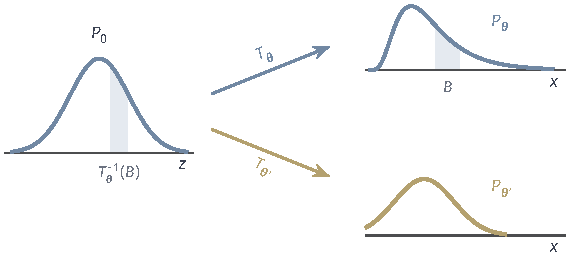
\includegraphics[width=96.6mm]{figures/07-probability/04-distribution-analysis/tikz/dfam-pushforward-scheme/figure.pdf}
  \caption{推前族的结构。左：固定的基础分布$P_0$，浅蓝带是集合$T_{\bm{\theta}}^{-1}(B)$；中间：随参数变化的映射$T_{\bm{\theta}}$；右：输出分布$P_{\bm{\theta}}$，浅蓝带是$B$。两块浅蓝区域的概率相等。两个参数$\bm{\theta}$、$\bm{\theta}'$（蓝、黄）共用同一个$P_0$。}
  \label{fig:dfam-pushforward-scheme}
\end{BookInlineFigure}

这种描述有两个直接的好处。第一，期望可以在基础空间上计算：对使下式一端有意义的可测函数$g$，
\begin{equation}
  \mathbb{E}_{P_{\bm{\theta}}}[g]=\mathbb{E}\bigl[g\bigl(T_{\bm{\theta}}(Z)\bigr)\bigr],
  \label{eq:dfam-pushforward-expectation}
\end{equation}
这是推前测度的积分公式，见\BookChapterRef{chap:pushforward-measures}{卷四第9章“推前测度”}。第二，生成样本只需生成$Z$再算一次映射。两者都不要求$P_{\bm{\theta}}$有密度。

推前构造的表达能力很强。第~\ref{chap:random-variables}章证明，若$U\sim\operatorname{Unif}(0,1)$，$Q$是任一分布函数$F$的分位数函数，则$Q(U)$的分布函数是$F$。所以$\mathbb{R}$上每一个分布都是$\operatorname{Unif}(0,1)$的推前。真正限制一个推前族的，是允许的映射类；下面两小节分别看最简单的映射类，以及映射怎样改变分布的结构。

\subsection{位置尺度族}
\label{sec:dfam-location-scale}

最简单的映射是平移加正向伸缩。第~\ref{chap:common-distributions}章已经用它解释过位置参数与尺度参数，这里把它作为推前族整理一遍，看分布函数、分位数和矩怎样随参数变化。

\begin{definition}[位置尺度族]
\label{def:dfam-location-scale}
设$Z$是实值随机变量，分布为$P_0$。对$\mu\in\mathbb{R}$、$\sigma>0$，令$P_{\mu,\sigma}$为$\mu+\sigma Z$的分布。$\{P_{\mu,\sigma}:\mu\in\mathbb{R},\ \sigma>0\}$称为由$P_0$生成的\term{位置尺度族}（location-scale family）。
\end{definition}

\paragraph{分布函数与分位数}
记$X=\mu+\sigma Z$。由$\sigma>0$，事件$\{X\leq x\}$与$\{Z\leq(x-\mu)/\sigma\}$相同，所以
\begin{equation}
  F_X(x)=F_Z\Bigl(\frac{x-\mu}{\sigma}\Bigr).
  \label{eq:dfam-ls-cdf}
\end{equation}
分布函数的图像只是被横向平移和伸缩。分位数函数的变化方向相反：第~\ref{chap:random-variables}章对$a>0$证明了$aZ+b$的分位数函数是$aQ_Z+b$，取$a=\sigma$、$b=\mu$，得到
\begin{equation}
  Q_X(u)=\mu+\sigma Q_Z(u),\qquad 0<u<1 .
  \label{eq:dfam-ls-quantile}
\end{equation}

式~\eqref{eq:dfam-ls-quantile}对每个$u$都成立，所以中位数、四分位数这些分位数一起按同一个仿射映射变化，四分位距乘以$\sigma$。把$X$的分位数对$Z$的同一水平分位数作图，点$(Q_Z(u),Q_X(u))$全部落在斜率为$\sigma$、截距为$\mu$的直线上。这条直线是检验“$X$是否属于$P_0$生成的位置尺度族”的图形办法，它不需要任何矩存在。

\paragraph{矩与标准化形状}
若$\mathbb{E}\lvert Z\rvert^{k}<\infty$，由凸函数$t\mapsto\lvert t\rvert^{k}$（$k\geq1$）的Jensen不等式，
\[
  \lvert X\rvert^{k}\leq2^{k-1}\bigl(\lvert\mu\rvert^{k}+\sigma^{k}\lvert Z\rvert^{k}\bigr),
\]
所以$X$的$k$阶矩也有限。由期望的线性和方差的缩放规律，
\begin{equation}
  \mathbb{E}[X]=\mu+\sigma\,\mathbb{E}[Z],\qquad\operatorname{Var}(X)=\sigma^{2}\operatorname{Var}(Z).
  \label{eq:dfam-ls-moments}
\end{equation}
矩不存在时，这些式子没有意义，但式~\eqref{eq:dfam-ls-cdf}与式~\eqref{eq:dfam-ls-quantile}照样成立。

再看偏度与峰度这类描述形状的量。设$\operatorname{Var}(Z)>0$，记$m_Z=\mathbb{E}[Z]$，$s_Z$为$Z$的标准差。由式~\eqref{eq:dfam-ls-moments}，$X$的标准化变量是
\[
  \frac{X-\mathbb{E}[X]}{\sqrt{\operatorname{Var}(X)}}=\frac{\sigma(Z-m_Z)}{\sigma s_Z}=\frac{Z-m_Z}{s_Z} .
\]
它与$\mu,\sigma$无关，所以只要相应的矩存在，标准化后的各阶矩，特别是偏度与峰度，在整个位置尺度族中保持不变。

更直接地，$(X-\mu)/\sigma=Z$，把族中任一成员按自己的参数标准化，都回到同一个基础分布。位置与尺度只决定分布放在哪里、铺开多宽，不改变标准化后的形状。

\paragraph{密度}
若$Z$有密度$f_Z$，第~\ref{chap:common-distributions}章已经算出$X$的密度
\begin{equation}
  f_X(x)=\frac{1}{\sigma}\,f_Z\Bigl(\frac{x-\mu}{\sigma}\Bigr).
  \label{eq:dfam-ls-density}
\end{equation}
因子$1/\sigma$来自伸缩：质量不变而区间拉长$\sigma$倍，单位长度上的质量就降为$1/\sigma$。

\paragraph{一个完整的例子}
取基础分布$Z\sim\operatorname{Exp}(1)$。由式~\eqref{eq:dfam-ls-cdf}，$X=\mu+\sigma Z$的分布函数是
\[
  F_X(x)=1-\exp\Bigl(-\frac{x-\mu}{\sigma}\Bigr),\qquad x\geq\mu ,
\]
$x<\mu$时为$0$。它的支撑是$[\mu,\infty)$，左端点随位置参数移动。$Z$的分位数函数是$Q_Z(u)=-\ln(1-u)$，由式~\eqref{eq:dfam-ls-quantile}，
\[
  Q_X(u)=\mu-\sigma\ln(1-u).
\]

取$\mu=1$、$\sigma=2$。中位数与两个四分位数分别是
\[
  Q_X(\tfrac12)=1+2\ln2\approx2.386,\quad Q_X(\tfrac14)\approx1.575,\quad Q_X(\tfrac34)\approx3.773 .
\]
四分位距是$2(\ln4-\ln\tfrac43)=2\ln3\approx2.197$，正好是$Z$的四分位距$\ln3$的$\sigma=2$倍。由式~\eqref{eq:dfam-ls-moments}，均值与方差是
\[
  \mathbb{E}[X]=1+2\cdot1=3,\qquad\operatorname{Var}(X)=4\cdot1=4 .
\]
$\operatorname{Exp}(1)$的偏度是$2$，所以族中每个成员的偏度都是$2$。

图~\ref{fig:dfam-location-scale}(a)画出三组参数的密度，它们看上去宽窄、位置都不同；(b)是分位数对照，三条曲线都是直线，斜率与截距读出$\sigma$与$\mu$。直线的事实说明它们属于同一个位置尺度族，宽窄的差别只是刻度的差别。

\begin{BookInlineFigure}
  \centering
  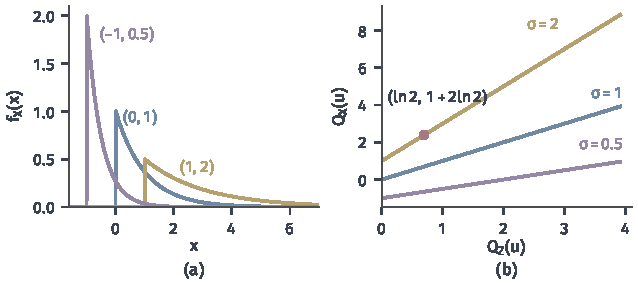
\includegraphics[width=108mm]{figures/07-probability/04-distribution-analysis/matplotlib/dfam-location-scale/figure.pdf}
  \caption{由$\operatorname{Exp}(1)$生成的位置尺度族。(a)$(\mu,\sigma)=(0,1)$（蓝）、$(1,2)$（黄）、$(-1,0.5)$（紫）的密度，支撑的左端点在$x=\mu$。(b)各成员的分位数$Q_X(u)$对基础分位数$Q_Z(u)$作图，$u$取$0.02$到$0.98$，得到斜率$\sigma$、截距$\mu$的直线；红点是$(\mu,\sigma)=(1,2)$的中位数$(\ln2,\ 1+2\ln2)$。}
  \label{fig:dfam-location-scale}
\end{BookInlineFigure}

\paragraph{基础分布的约定与参数的唯一性}
同一个位置尺度族可以由不同的基础分布生成。$\mathcal{N}(0,1)$与$\mathcal{N}(0,4)$生成的族都是全体高斯分布，但在后一种约定下，$\mu+\sigma Z$的标准差是$2\sigma$，同一个数字$\sigma$表示的宽度不同。一般地，$P_0$换成$a+bZ$（$b>0$）的分布，生成的族不变，参数按$(\mu,\sigma)\mapsto(\mu-\sigma a/b,\ \sigma/b)$换算。所以谈论位置和尺度参数的数值时，必须先固定基础分布。

固定基础分布以后，若$Z$不是几乎必然的常数，参数$(\mu,\sigma)$就是可辨识的。这时$Q_Z$不是常函数，可以取$u<v$使$Q_Z(u)<Q_Z(v)$。若$P_{\mu,\sigma}=P_{\mu',\sigma'}$，两者的分位数函数相同，由式~\eqref{eq:dfam-ls-quantile}，
\[
  \mu+\sigma Q_Z(u)=\mu'+\sigma'Q_Z(u),\qquad\mu+\sigma Q_Z(v)=\mu'+\sigma'Q_Z(v).
\]
两式相减得$(\sigma-\sigma')(Q_Z(v)-Q_Z(u))=0$，于是$\sigma=\sigma'$，再代回得$\mu=\mu'$。若$Z$是常数$c$，则$P_{\mu,\sigma}=\delta_{\mu+\sigma c}$，只有和$\mu+\sigma c$可见，参数不可辨识，这正是上一节$\mathcal{N}(\theta_1+\theta_2,1)$那类冗余的极端情形。

\paragraph{没有矩的成员}
Cauchy分布$f_Z(z)=1/(\pi(1+z^{2}))$没有均值。它生成的位置尺度族中，$\mu$不是均值，$\sigma$也不是标准差，但由$F_Z(z)=\tfrac12+\tfrac1\pi\arctan z$得$Q_Z(\tfrac14)=-1$、$Q_Z(\tfrac34)=1$，再由式~\eqref{eq:dfam-ls-quantile}，$\mu$是中位数，四分位距是$2\sigma$。位置尺度族的定义本身只用到映射，矩只是在存在时顺带跟着变化。

这个族的局限也很清楚：它永远改变不了标准化后的形状。由$\mathcal{N}(0,1)$生成的族里没有偏斜的分布，由$\operatorname{Exp}(1)$生成的族里偏度永远是$2$。要改变形状，映射必须不再是仿射的。

\subsection{映射对分布结构的影响}
\label{sec:dfam-map-effects}

仿射映射只做平移和伸缩。一般映射可以把基础分布弯曲、压扁或切碎，相应地改变输出分布的形状、支撑的维数，甚至让连续分布长出点质量。下面依次看三类映射：可逆的非线性映射、降低维数的映射和离散化。

\paragraph{可逆非线性映射改变形状}
取基础变量$Z\sim\mathcal{N}(0,1)$与映射$T_{\mu,\sigma}(z)=\exp(\mu+\sigma z)$，$\sigma>0$。它是$\mathcal{N}(0,1)$生成的位置尺度族再接一个固定的指数函数，输出是第~\ref{chap:random-variable-transformations}章的对数正态分布。指数函数把$\mathbb{R}$一一地送到$(0,\infty)$，导数处处为正，所以可以用一元单调换元公式求密度：
\[
  f_X(x)=\frac{1}{\sigma x}\,\varphi\Bigl(\frac{\ln x-\mu}{\sigma}\Bigr),\qquad x>0 .
\]

参数的角色在这里发生了变化。$X=\mathrm{e}^{\mu}\,(\mathrm{e}^{Z})^{\sigma}$，原来的位置参数$\mu$变成乘法因子$\mathrm{e}^{\mu}$，即对数正态族的尺度参数；原来的尺度参数$\sigma$成了指数$(\mathrm{e}^{Z})^{\sigma}$中的幂次，它改变的是形状。由高斯的矩母函数，
\[
  \mathbb{E}[X^{k}]=\mathrm{e}^{k\mu}\,\mathbb{E}[\mathrm{e}^{k\sigma Z}]=\mathrm{e}^{k\mu+k^{2}\sigma^{2}/2}.
\]
把$k=1,2,3$代入偏度的定义，因子$\mathrm{e}^{\mu}$全部约去，得到对数正态分布的偏度
\[
  (\mathrm{e}^{\sigma^{2}}+2)\sqrt{\mathrm{e}^{\sigma^{2}}-1},
\]
$\sigma=0.25$时约为$0.78$，$\sigma=1$时约为$6.18$。图~\ref{fig:dfam-lognormal-map}(a)画出映射本身：$z$轴上等概率的区间被送到长短悬殊的区间，右侧被拉长，左侧被压缩；(b)是固定$\mu=0$（中位数为$1$）时三个$\sigma$的密度，$\sigma$越大越偏斜。

\begin{BookInlineFigure}
  \centering
  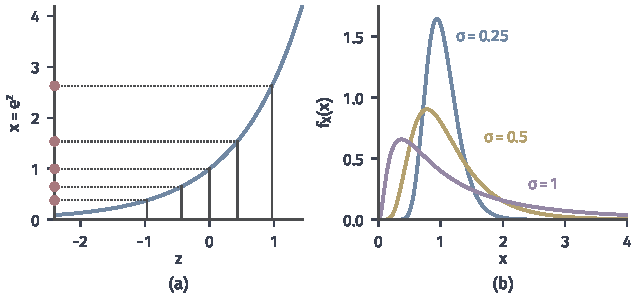
\includegraphics[width=108mm]{figures/07-probability/04-distribution-analysis/matplotlib/dfam-lognormal-map/figure.pdf}
  \caption{可逆非线性映射改变形状。(a)映射$x=\mathrm{e}^{z}$（蓝线）；横轴上深灰竖线把$\mathcal{N}(0,1)$分成六段等概率区间，分点经映射后在纵轴上的位置用红点标出，等概率区间的长度在$x$方向右侧拉长、左侧压缩。(b)$\mu=0$时$\sigma=0.25$（蓝）、$0.5$（黄）、$1$（紫）的对数正态密度，三者中位数都是$1$。}
  \label{fig:dfam-lognormal-map}
\end{BookInlineFigure}

换元公式在这里成立，靠的是映射同维、可逆、连续可微且导数不为零，第~\ref{chap:random-variable-transformations}章与\BookChapterRef{chap:pushforward-measures}{卷四第9章“推前测度”}都要求这些条件。条件破坏时，推前分布依然由式~\eqref{eq:dfam-pushforward}完全确定，只是不再有这样一个公式，甚至根本没有密度。下面两类映射就是这样。

\paragraph{把低维随机性放进高维空间}
取$Z\sim\operatorname{Unif}(0,1)$，参数$r>0$，令
\[
  \bm{X}_r=\bigl(r\cos(2\pi Z),\ r\sin(2\pi Z)\bigr).
\]
$\bm{X}_r$在半径为$r$的圆周上均匀分布，以概率$1$落在圆周上。圆周的平面面积为零，所以$\bm{X}_r$的分布不相对平面Lebesgue测度绝对连续，没有二维密度。参数$r$在这里控制的是支撑本身：不同的$r$给出的分布落在互不相交的圆周上。

这不是圆周的特殊性质。只要输入的维数低于输出，光滑映射的像就是零测集。

\begin{lemma}[低维像的零测性]
\label{lem:dfam-low-dim-image}
设$k<d$，$T:\mathbb{R}^{k}\to\mathbb{R}^{d}$连续可微。则$T(\mathbb{R}^{k})$是$\mathbb{R}^{d}$中的Borel集，且Lebesgue测度为零。因此对$\mathbb{R}^{k}$上任一概率测度$P_0$，$T_\#P_0$都没有相对$d$维Lebesgue测度的密度。
\end{lemma}

\begin{proof}
固定$R>0$，记$K_R=[-R,R]^{k}$。$K_R$是紧凸集，$DT$在$K_R$上连续，所以算子范数有上界$L$。由中值不等式，对$\bm{z},\bm{z}'\in K_R$，
\[
  \lVert T(\bm{z})-T(\bm{z}')\rVert_2\leq L\lVert\bm{z}-\bm{z}'\rVert_2 .
\]

把$K_R$等分成$m^{k}$个边长为$2R/m$的小立方体，每个的直径是$2R\sqrt{k}/m$。它的像落在半径为$2LR\sqrt{k}/m$的球内，从而落在边长为$4LR\sqrt{k}/m$的立方体内。把$m^{k}$块的体积加起来，
\[
  \lambda_d\bigl(T(K_R)\bigr)\leq m^{k}\Bigl(\frac{4LR\sqrt{k}}{m}\Bigr)^{d}=(4LR\sqrt{k})^{d}\,m^{k-d} .
\]
这里$T(K_R)$是紧集的连续像，仍是紧集，所以可测。由$k<d$，令$m\to\infty$，右边趋于零，所以$\lambda_d(T(K_R))=0$。

取$R=1,2,\dots$，$T(\mathbb{R}^{k})=\bigcup_RT(K_R)$是可数个紧集之并，是Borel集，测度为零。$T_\#P_0$在这个零测集上的质量是$P_0(\mathbb{R}^{k})=1$，所以它不相对$\lambda_d$绝对连续，没有密度。
\end{proof}

降维的方向相反时情况不同。$\bm{Z}\sim\mathcal{N}(\bm{0},\bm{I}_2)$，$X=Z_1+Z_2$把两个坐标并成一个，输出有密度，它是$\mathcal{N}(0,2)$；但这个密度不能用同维换元求得，要沿被合并的方向积分，即第~\ref{chap:random-variable-transformations}章的卷积。决定有没有密度的不是输入输出的维数谁大，而是映射是否把正的质量压进输出空间的零测集。线性映射$\bm{X}=\bm{A}\bm{Z}$中$\bm{A}$为奇异的$2\times2$矩阵时，像是一条直线，正是第~\ref{chap:multivariate-distributions}章退化高斯的情形。

\paragraph{离散化产生原子}
第三类映射把连续值归到有限或可数个格子里。取$Z\sim\mathcal{N}(0,1)$，位置参数$\mu$，令$X=\operatorname{round}(\mu+Z)$为最接近$\mu+Z$的整数（半整数处的取法不影响分布，因为那是零概率事件）。$X=k$当且仅当$k-\tfrac12\leq\mu+Z<k+\tfrac12$，所以
\begin{equation}
  \mathbb{P}(X=k)=\Phi\bigl(k+\tfrac12-\mu\bigr)-\Phi\bigl(k-\tfrac12-\mu\bigr),\qquad k\in\mathbb{Z}.
  \label{eq:dfam-rounding}
\end{equation}
连续的基础分布被推成一张概率表。取$\mu=0.3$，代入式~\eqref{eq:dfam-rounding}，
\[
  \mathbb{P}(X=-1)\approx0.176,\quad\mathbb{P}(X=0)\approx0.367,\quad\mathbb{P}(X=1)\approx0.306 .
\]

离散化也可以只作用在一部分取值上。令$X=\max(\mu+Z,0)$，负的读数都记成$0$。$\{X=0\}=\{Z\leq-\mu\}$，于是$\mathbb{P}(X=0)=\Phi(-\mu)$，$X$在$0$处有一个原子；在$(0,\infty)$上$X=\mu+Z$，有密度$\varphi(x-\mu)$。这个分布既不是概率表，也没有相对Lebesgue测度的密度。若取参考测度$\nu=\delta_0+\lambda_1$，它相对$\nu$的密度是
\[
  p(0)=\Phi(-\mu),\qquad p(x)=\varphi(x-\mu)\quad(x>0).
\]
$\mu=0.5$时原子的质量是$\Phi(-0.5)\approx0.309$。

\begin{BookInlineFigure}
  \centering
  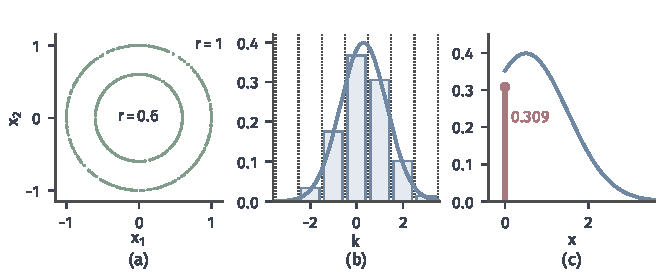
\includegraphics[width=112mm]{figures/07-probability/04-distribution-analysis/matplotlib/dfam-map-effects/figure.pdf}
  \caption{映射改变支撑与类型。(a)$Z\sim\operatorname{Unif}(0,1)$经$z\mapsto r(\cos2\pi z,\sin2\pi z)$得到的$400$个点（绿），$r=1$与$r=0.6$；分布全部落在圆周上，没有平面密度。(b)$\mu=0.3$时$\operatorname{round}(\mu+Z)$的概率表（浅蓝柱），蓝线是$\mu+Z$的密度，深灰竖线是格子边界$k\pm\tfrac12$。(c)$\max(\mu+Z,0)$，$\mu=0.5$：$(0,\infty)$上的密度（蓝线）与$0$处质量$0.309$的原子（红色竖线）。}
  \label{fig:dfam-map-effects}
\end{BookInlineFigure}

图~\ref{fig:dfam-map-effects}把三种结构放在一起。圆周上的分布支撑退化，取整得到概率表，截断得到原子与密度并存的混合类型。三者都是从有密度的基础分布出发、经过可测映射得到的，所以推前族的成员可以有任何类型；只有在同维可逆光滑的情形，才能放心地把它写成一个普通的密度模型。描述一般推前族时，应当用式~\eqref{eq:dfam-pushforward}和式~\eqref{eq:dfam-pushforward-expectation}，而不是先假定存在密度。
